Il modello di sviluppo adottato si ispira a quello \textbf{incrementale} secondo ISO/IEC 12207:1995, cosicché possano essere garantite la qualità e la conformità attese durante lo svolgimento del progetto.

\subsection{Il modello di sviluppo}
Nel modello incrementale, il numero di incrementi viene pianificato in base ai requisiti identificati durante l'analisi. Essi vengono ordinati in base alla loro priorità che viene determinata in base all'importanza strategica.\\
Dopo di che, si passa alla suddivisione dei requisiti nei vari incrementi. Chiaramente, quelli più incombenti, ovvero quelli a priorità più alta, saranno assegnati ai primi incrementi dell'iterazione. In tal modo, il prodotto viene consegnato al committente incrementalmente tramite Proof of Concept.\\
Durante gli incrementi, non può essere aggiunto o modificato alcun requisito. Se ciò dovesse essere necessario, il requisito verrà aggiunto a quelli dell'incremento successivo. Una volta completato il suo sviluppo, esso viene aggiunto al prodotto.\\
La scelta del modello incrementale aiuta la definizione dei requisiti, che sono il punto critico del progetto. Infatti, la proponente non ha posto vincoli particolarmente stringenti sulle tecnologie da impiegare: ciò da un lato permette una certa libertà di azione al team, dall'altro non permette un'identificazione veloce dei requisiti tecnologici. Il modello incrementale prevede nell'ordine l'analisi dei requisiti del sistema, la progettazione architetturale del sistema, l'analisi dei requisiti software e, infine, la progettazione architetturale del software. Lo svolgimento di attività di progettazione prima del completamento dell'analisi permetterà la determinazione dei requisiti tecnologici non ancora identificati.

\subsubsection{Organizzazione del modello}
Il modello adottato è composto da 5 periodi principali (e spesso sovrapposti):
\begin{enumerate}
	\item \textbf{Avvio} (2018-12-4 - 2018-12-17): durante questo periodo, tutti i membri sono impegnati nella ricerca degli strumenti adatti al compimento delle prime attività. Concluso questo periodo, si attende che siano completate le versioni di base (v0.1.0) delle \textit{Norme di progetto} e del \emph{Piano di progetto} in modo da poter svolgere i processi successivi in maniera ordinata e regolamentata.
	\item \textbf{Analisi dei Requisiti e Progettazione architetturale} (2018-12-17 - 2019-02-18): all'inizio del periodo, vengono effettuate delle aggiunte alle \textit{Norme di progetto} e al \textit{Piano di progetto}. Inoltre, viene definito e verificato il \textit{Piano di qualifica}. Contestualmente, viene avviata l'analisi dei requisiti del sistema. Successivamente dovranno essere aggiornati \textit{Piano di qualifica} e di \textit{Piano di progetto} con i rispettivi rendiconti. Durante questo periodo, è prevista la Revisione dei Requisiti che determinerà l'ingresso o l'esclusione temporanea del gruppo dal progetto didattico. Successivamente, vengono effettuate le aggiunte necessarie alla normazione (\textit{Norme di progetto}) e alla verifica (\textit{Piano di qualifica}) del processo di progettazione. Inoltre, vengono fatti degli aggiustamenti alla pianificazione di progetto in base agli scostamenti rilevati. Segue una prima attività di progettazione architetturale, seguita a sua volta dall'analisi dei requisiti software. Alla fine di quest'ultima attività, l'analisi dei requisiti si potrà dire completa e ciò permetterà di proseguire con ulteriori incrementi di progettazione architetturale. 
\item \textbf{Progettazione di dettaglio} (2019-02-14 - 2019-04-21): il periodo inizia con incrementi di progettazione di dettaglio intervallati da attività di codifica (appartenenti alla realizzazione), in modo da poter progettare e realizzare incrementalmente il sistema. Durante questo periodo è prevista la Revisione di Progettazione. Tuttavia, sono previsti degli incrementi per la progettazione di dettaglio successivi alla revisione.
	\item \textbf{Realizzazione} (2019-02-21 - 2019-04-27): all'inizio del periodo è previsto un incremento alla normazione e ai piani per le attività di realizzazione. Dopo di che, sono presenti diversi incrementi per la codifica, intervallati da attività di progettazione di dettaglio in modo da poter produrre incrementalmente il sistema. Durante questo periodo avviene la Revisione di Qualifica, prima della quale vengono svolti degli incrementi ai piani. Segue un incremento di codifica.
	\item \textbf{Validazione} (2019-04-13 - 2019-05-17): all'inizio del periodo, vengono aggiunte le norme necessarie alla validazione, viene completato il Piano di Qualifica e viene modificato il \textit{Piano di progetto} in base agli scostamenti. Seguono, dunque, i test di qualifica. Nel caso in cui tali test abbiano esito negativo è possibile correre ai ripari tramite attività di progettazione e codifica. Una volta che il test di qualifica ha esito positivo, è possibile procedere al collaudo. Segue la produzione del manuale, l'aggiunta della rendicontazione nel \textit{Piano di qualifica} e nel \textit{Piano di progetto}. Infine, il prodotto viene consegnato.
\end{enumerate}

\begin{figure}[h]
	\centering
	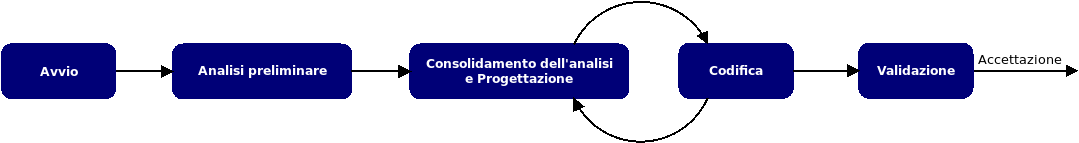
\includegraphics[scale=0.4]{images/Model/model.png}
	\caption{Ciclo di vita}
\end{figure}

\subsection{Attività}
Ogni incremento prevede delle attività. Ognuna di esse viene assegnata dal responsabile a uno dei membri del team di sviluppo, il quale svolgerà il lavoro assegnato. Una volta completato, il lavoro dovrà essere sottoposto a verifica.\\
Nel caso in cui il risultato sia soddisfacente, l'attività è considerata conclusa e il responsabile potrà assegnarne una nuova al membro.\\ 
In caso contrario, il lavoro non è considerato completato e lo sviluppatore dovrà correggere dove indicato durante l'incremento successivo. Le correzioni effettuate dovranno essere a loro volta verificate.\\
La quantità di giorni lavorativi per ciascuna attività varia dai 5 ai 10 giorni dipendentemente dalla sua complessità.

\begin{figure}[h]
	\centering
	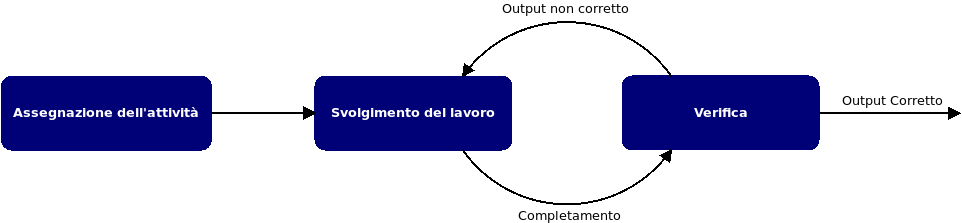
\includegraphics[scale=0.45]{images/Model/activity.png}
	\caption{Ciclo di un'attività}
\end{figure}
